\section{Theorie}
\label{sec:Theorie}
Mit Drehmoment $\vec{M}$ Trägheitsmoment $I$ und Winkelbeschleunigung $\dot{\omega}$
lassen sich Dynamische Rotationsbewegungen beschreiben. Das Trägheitsmoment ist
durch
\begin{equation}
  I=\sum_i r_1^2m_i=\int_{}^{} r^2 \text{d}m
\end{equation}
gegeben.
Beispiele für Trägheitsmomente sind in der Abbildung \ref{fig:Traegheitsmomente}
dargestellt.
\begin{figure}
  \centering
  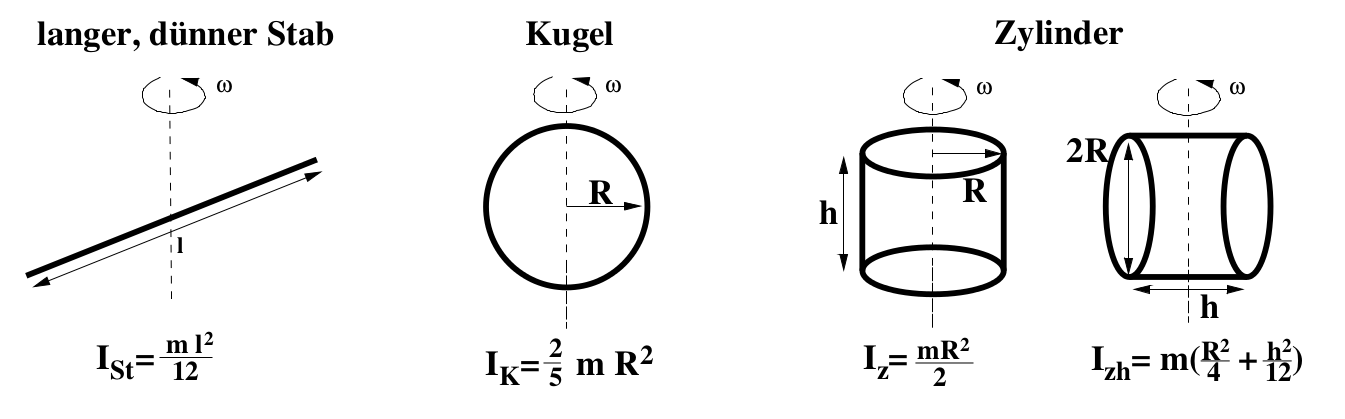
\includegraphics[width=0.9\textwidth]{Traegheitsmomente.png}
  \caption{Trägheitsmomente für verschiedene Körper \cite{sample}.}
  \label{fig:Traegheitsmomente}
\end{figure}
Ist ein Körper, dessen Trägheitsmoment bei Rotation um die Schwerpunktsachse
bekannt ist, von der Drehachse durch seinen Schwerpunkt um den Abstand $a$
verschoben, so lässt sich das neue Trägheitsmoment mit dem Steinerschen Satz
\begin{equation}
  I=I_s+m a^2
  \label{eqn:steiner}
\end{equation}
berechnen. Das Drehmoment M berechnet sich durch
\begin{equation}
  \vec{M}=\vec{F}\times\vec{r}\;\;.
\end{equation}
Wenn in einem System eine zum Auslenkungswinkel $\varphi$ Rücktreibende Kraft
existiert, führt das System eine Schwingung aus mit der Schwingungsdauer
\begin{equation}
  T=2\pi\sqrt{\frac{I}{D}}\;\;.
  \label{eqn:Periodetorrosion}
\end{equation}
Diese Gleichung gilt mit der Näherung für kleine Winkel.
Das durch die rücktreibende Kraft erzeugte Drehmoment ist bestimmt durch
\begin{equation}
  M=D \varphi\;\;.
  \label{eqn:Traegheitmomenttorrosion}
\end{equation}
gegeben. Mit den Gleichungen \eqref{eqn:Traegheitmomenttorrosion} und
\eqref{eqn:Periodetorrosion} lassen sich auch die Winkelrichtgrößen $D$ von
Torsionsfedern berechnen.
\begin{equation}
  D=\frac{Fr}{\varphi}
  \label{eqn:Winkelrichtgroesse}
\end{equation}
\cite{sample}
